\documentclass{lecturenotes}

\renewcommand{\vecka}{2}

\setbeamertemplate{footline}[frame number]
\title[Föreläsningsanteckningar EDA016, 2015]{EDA016 Programmeringsteknik för D}
\subtitle{Läsvecka \vecka: Kodstruktur}
\author{Björn Regnell}
\institute{Datavetenskap, LTH}
\date{Lp1-2, HT 2015}
 
\begin{document}

\frame{\titlepage}
\setnextsection{2}
\section[Vecka \vecka: Kodstruktur]{Kodstruktur}
\frame{\tableofcontents}

%%%%%%%%%%%%%%%%%%%%%%%%%%%%%%%%%%%%%%

\subsection{Att göra denna vecka}

\begin{Slide}{Resurstider och Labbar}
\begin{itemize}
\item Laborationer är \Alert{obligatoriska}.\\ Ev. sjukdom måste anmälas \Alert{före} till kursansvarig!
\item Resurstiderna hade närvaro på endast ca. 50\%. 
   \\Varför?
\end{itemize}
\end{Slide}
%%%
\frame{\frametitle{Att göra i Vecka \vecka: Fatta kodstruktur}
\begin{enumerate}
\item Läs följande kapitel i kursboken: \\ 2.1-2.6, 4, 5.4, 7.2, 7.5-7.6, 7.8-7.9; 
 Begrepp: \\algoritm, pseudokod, abstraktion, oändlig loop,while-sats, for-sats, paket, import, referensvariabel, objekt, referenstilldelning, referenslikhet 
\item Gör övning 2: Paket, kodfiler, och dokumentation
\item OBS! Ingen lab denna vecka
\item Träffas i samarbetsgrupper och hjälp varandra att förstå
\item Gör klart \href{https://github.com/bjornregnell/lth-eda016-2015/tree/master/assignments}{samarbetskontrakt} och visa för handledare på resurstid
\item \Alert{Koda på resurstiderna} och få hjälp och tips! \\ Varför var de så få kom kom till resurstiderna vecka 1?
\end{enumerate}
}

\subsection{Algoritmer}

\begin{Slide}{Vad är en algoritm?}
En \href{https://sv.wikipedia.org/wiki/Algoritm}{algoritm} är en sekvens av instruktioner\\ som beskriver hur man löser ett problem \\
\vspace{2em}
Exempel: \\ ~matrecept \\ \pause ~uppdatera highscore i ett spel \\ ~...
\begin{tikzpicture}[overlay]
\node[xshift=0.8\textwidth, scale=1.6] at (0,0) {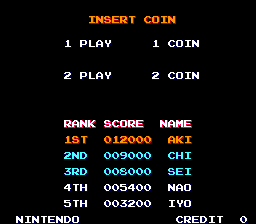
\includegraphics[width=0.25\textwidth]{img/highscore}};
\end{tikzpicture}
\end{Slide}

\begin{Slide}{Algoritm-exempel: Highscore}
\Emph{Problem}: Uppdatera high-score i ett spel \\ \vspace{1em}

\Emph{Varför?} \pause Så att de som spelar uppmuntras att spela mer :) \\ \vspace{1em}

\Emph{Algoritm:}\pause
\begin{enumerate}
\item $points$ $\leftarrow$ poängen efter senaste spelet
\item $highscore$ $\leftarrow$ bästa resultatet innan senaste spelet
\item \Key{om} $points$ är större än $highscore$ 
\begin{enumerate}[ ~~]
\item  Skriv ''Försök igen!''
\end{enumerate}
\Key{annars}
\begin{enumerate}[ ~~]
\item  Skriv ''Grattis!''
\end{enumerate}
\end{enumerate}
\pause
\scriptsize \Alert{Hittar du buggen?}
\end{Slide}

\begin{Slide}{Algoritm-exempel: Highscore}
\lstinputlisting[language=Java, numbers=left]{../examples/terminal/highscore/HighScore.java}
Är det en bugg eller en feature att det står\\ \texttt{(points > highscore} och inte \texttt{points >= highscore} ?
% Buggen är att man inte får GRATTIS om poäng == highscore vilket är tråkigt :)
\end{Slide}

\begin{Slide}{Abstraktion -- varför?}
\begin{itemize}
\item Dela upp problem i delproblem
\item Skapa ''byggblock'' av kod som kan återanvändas
\item Dölja komplexiteten i lösningar
\item Abstraktion är själva \Emph{essensen i all programmering}
\end{itemize}
\begin{lstlisting}
    public static void main(String[] args){
    	askUser();
    	updateHighscore();
    }
\end{lstlisting}
Kolla hela programmet här:\\ \href{https://github.com/bjornregnell/lth-eda016-2015/blob/master/lectures/examples/terminal/highscore/HighScoreAbstraction.java}{https://github.com/bjornregnell/lth-eda016-2015} \\
i filen: \scriptsize\texttt{lectures/examples/terminal/highscore/HighScoreAbstraction.java}
\end{Slide}

\begin{Slide}{Vår första algoritmkluring: SWAP}
\Emph{Problem}: läs in och byt plats på två tal i minnet \\ \vspace{1em}
\pause
\Emph{Algoritm:}
\begin{enumerate}
\item skapa en Scanner
\item  läs in x
\item  läs in y
\item  Skriv ut x och y
\item  byt plats på värdena mellan x och y
\item  Skriv ut x och y
\end{enumerate}
\vspace{2em}
\footnotesize Varför kan det vara bra att kunna byta plats på olika värden? \\ \vspace{1em}\scriptsize
Steg 5 är egentligen en \Emph{abstraktion} av själva problemet SWAP, som inte är så lätt som det verkar och behöver delas upp i flera steg för att det ska vara rakt fram att översätta till exekverbar kod i t.ex. Java.
\end{Slide}


\begin{Slide}{Vår första algoritmkluring: SWAP}
\lstinputlisting[language=Java, numbers=left]{../examples/terminal/swap/SwapQuest.java}
\end{Slide}

\begin{Slide}{Vår första algoritmkluring: SWAP}
\lstinputlisting[language=Java, numbers=left]{../examples/terminal/swap/SwapSolution.java}
\footnotesize Övning: Rita hur minnet ser ut efter respektive raderna 7, 8, 12, 13, 14
\end{Slide}

\Subsection{Loop-strukturer}

\begin{Slide}{Mitt första program: en oändlig loop på ABC80}
\begin{columns}
\begin{column}{0.8\textwidth}
\begin{verbatim}
10 print "hej"
20 goto 10
\end{verbatim}
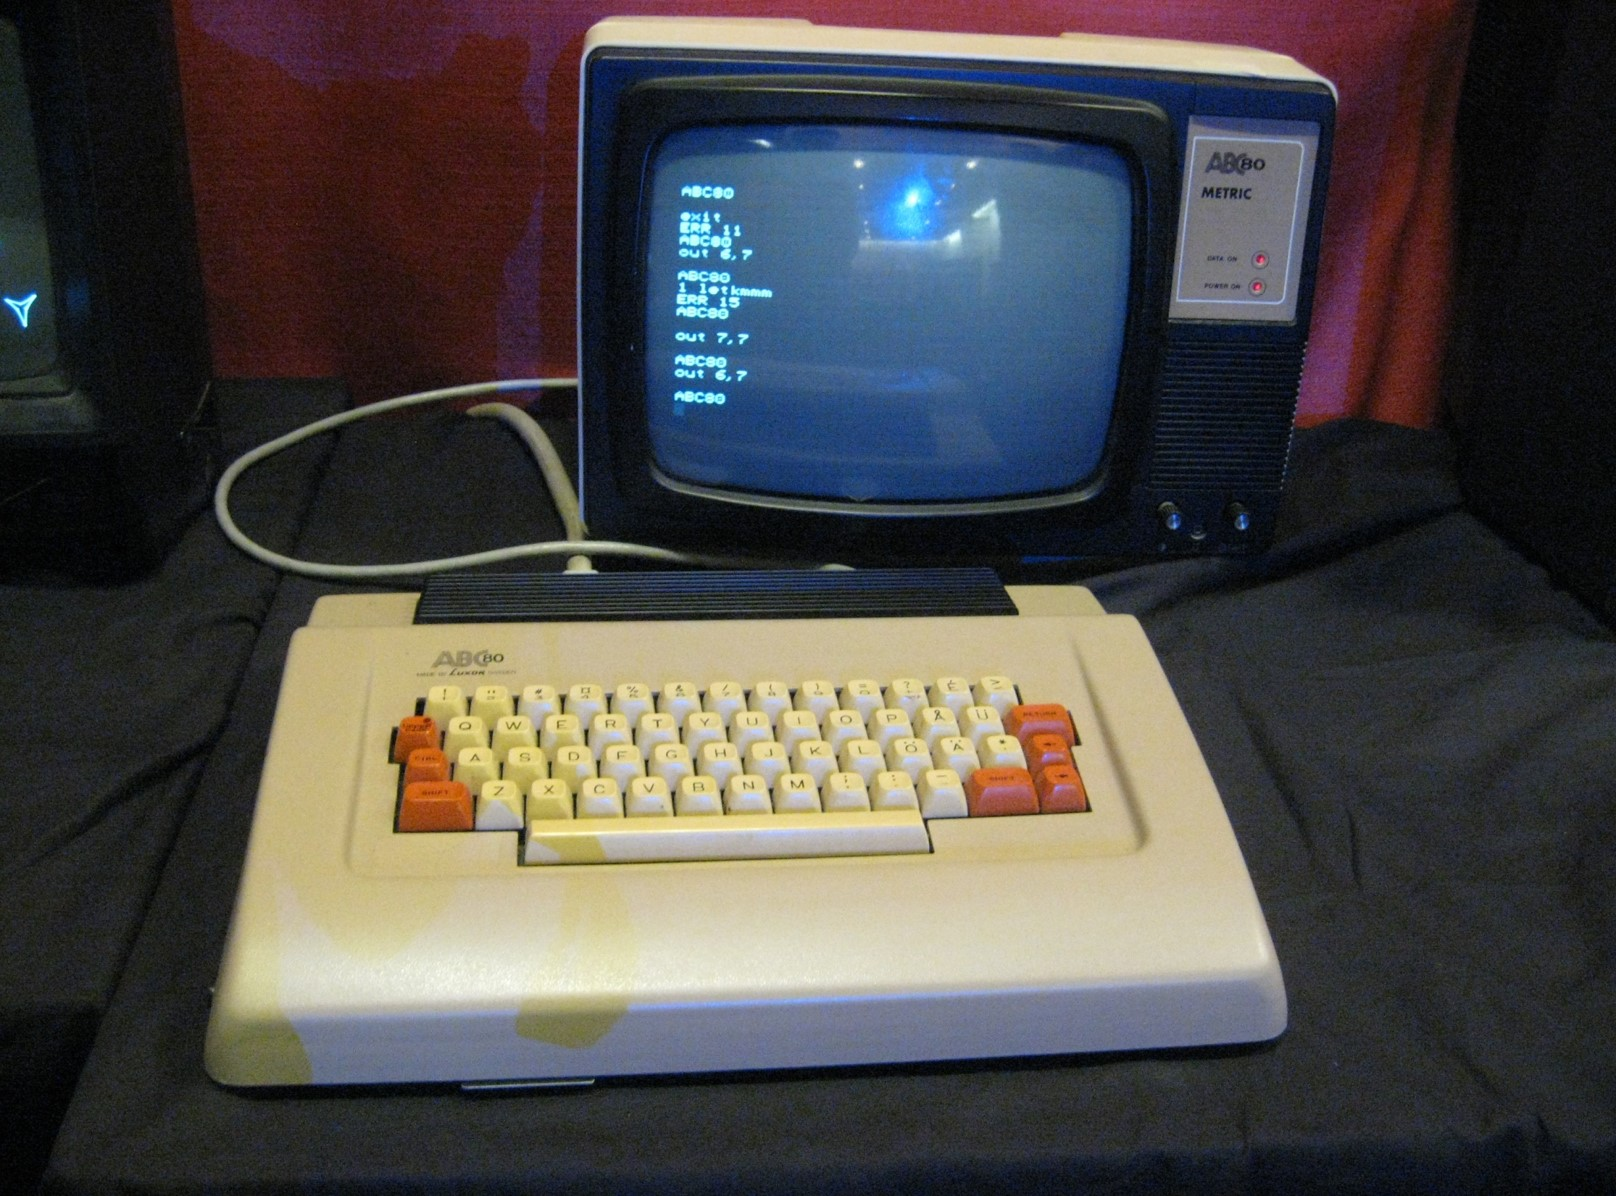
\includegraphics[width=0.8\textwidth]{img/abc80.jpg}
\end{column}
\begin{column}{0.3\textwidth}
\pause
\begin{verbatim}
hej
hej
hej
hej
hej
hej
hej
hej
hej
hej
hej
hej
<Ctrl+C>
\end{verbatim}

\end{column}
\end{columns}
\end{Slide}

\begin{Slide}{Repetition med while-sats}
\lstinputlisting[language=Java, numbers=left]{../examples/terminal/loops/InfiniteLoop.java}
\pause
\begin{itemize}
\item En av de saker en dator är \textit{extra} bra på är att göra samma sak om och om igen utan att tröttna! \\
Och det är ju människor \textit{extra} dåliga på :)
\item Med klockfrekvens i storleksordningen $10^9$ Hz är det ganska många instruktioner som kan göras per sekund...
\end{itemize}
\end{Slide}

\begin{Slide}{Oändlig while-loop med räknare}
\lstinputlisting[language=Java, numbers=left]{../examples/terminal/loops/InfiniteLoopWithCounter.java}
\end{Slide}

\begin{Slide}{Ändlig while-loop med räknare}
\lstinputlisting[language=Java, numbers=left]{../examples/terminal/loops/FiniteWhileLoopWithCounter.java}
\end{Slide}


\begin{Slide}{Ändlig for-loop med räknare}
\lstinputlisting[language=Java, numbers=left]{../examples/terminal/loops/ForLoop.java}
Denna sats är ekvivalent med föregående \Key{while}-sats.\footnote{\scriptsize Förutom att variabeln \texttt{i} finns efter \Key{while}-satsen men \textit{inte} efter \Key{for}-satsen }
\end{Slide}

\begin{Slide}{Ändlig while-loop med timer}
\lstinputlisting[language=Java, numbers=left]{../examples/terminal/loops/LoopWithTimer.java}
\scriptsize 
Övning: Skriv om till \Key{for}-loop och kolla om den är lika snabb som \Key{while}
\end{Slide}

\begin{Slide}{Algoritm: MIN/MAX}
\Emph{Problem}: hitta största talet \\ \vspace{1em}
\pause
\Emph{Algoritm:} 
\begin{enumerate}
\item $scan$ $\leftarrow$ en Scanner som läser det användaren skriver
\item $maxSoFar$ $\leftarrow$ ett heltal som är \textit{mindre} än alla andra heltal
\item  \Key{sålänge} det finns fler heltal att läsa: \\
~~ $x$ $\leftarrow$ läs in ett heltal med hjälp av $scan$ \\
~~ \Key{om} $x$ är större än $maxSoFar$ \\
~~~~~~ $maxSoFar$ $\leftarrow$ $x$
\item skriv ut $maxSoFar$ 
\end{enumerate}
\vspace{1em} \scriptsize 
Övning 1: Kör algoritmen med papper och penna med indata: \texttt{0~~41~~1~~45~~2~~3~~4}\\ 
Övning 2: skriv om så att algoritmen istället hittar \textit{minsta} talet.
\end{Slide}

\begin{Slide}{Övning: Implementera algoritmen MIN/MAX i Java}
\footnotesize
Några ledtrådar:
\begin{enumerate}
\item Man kan få det minsta heltalet med \href{https://docs.oracle.com/javase/8/docs/api/java/lang/Integer.html}{\lstinline{Integer.MIN_VALUE}} (negativt värde)
\item Man kan få det största heltalet med \href{https://docs.oracle.com/javase/8/docs/api/java/lang/Integer.html}{\lstinline{Integer.MAX_VALUE}}
\item Dokumentation av klassen \href{https://docs.oracle.com/javase/8/docs/api/java/util/Scanner.html}{Scanner} finns här: \url{https://docs.oracle.com/javase/8/docs/api/}
\item Man kan kolla om det finns mer att läsa med \href{https://docs.oracle.com/javase/8/docs/api/java/util/Scanner.html#hasNextInt--}{\lstinline{scan.hasNextInt()}}
\item Man läser nästa heltal med  \href{http://docs.oracle.com/javase/8/docs/api/java/util/Scanner.html#nextInt%28%29}{\lstinline{scan.nextInt()}}
\end{enumerate}
\vspace{2em}
\scriptsize Googlingstävling 1: Vem hittar först \underline{största} Double-värdet i Java? \\ Googlingstävling 2: Vem hittar först \underline{minsta} Double-värdet i Java?
% http://www.avajava.com/tutorials/lessons/how-do-i-find-the-max-and-min-values-of-primitive-types.html
\end{Slide}

%%%%%%%%%%%%%%%%%%%%%%%%%%%%%%%%%%%%%%
\subsection{Abstraktionsmekanismer}
\begin{Slide}{Varför kodstruktur med abstraktion?}
\begin{itemize}
\item Stora programdelar behöver delas upp annars blir det mycket svårt att förstå programmet.
\item Vi behöver kunna välja namn på saker i koden \textit{lokalt}, utan att det krockar med samma namn i andra delar av koden.
\item Abstraktioner hjälper till att hantera och kapsla in komplexa delar så att de blir enklare att använda om och om igen. \\Exempel på \Emph{abstraktionsmekanismer} i Java:
\begin{itemize}\footnotesize
\item \href{https://en.wikipedia.org/wiki/Java_package}{Paket} används för att organisera koddelar som samverkar i en hierarkisk katalogstruktur. Nyckelord: \Key{package}
\item \href{https://sv.wikipedia.org/wiki/Klass_\%28programmering\%29}{Klasser} är ''byggblock'' med kod som används för att skapa \href{https://sv.wikipedia.org/wiki/Objektorienterad_programmering\#Objekt}{objekt}, innehållande delar som hör ihop. Nyckelord: \Key{class}
\item \href{https://en.wikipedia.org/wiki/Method_\%28computer_programming\%29}{Metoder} är programdelar som finns i klasser och används för att lösa specifika uppgifter. Exempel: \texttt{updateHighScore()} 
\end{itemize}
\end{itemize}
\end{Slide}

\begin{Slide}{Exempel på olika sorters metoder:}
\begin{itemize}\footnotesize
\item \Emph{Procedurer} är metoder som \textit{gör} något men som inte returnerar något värde. Avsaknad av värde anges i Java med nyckelordet \Key{void}
\item \Emph{Funktioner} är metoder som beräknar och \textit{returnerar} ett specifikt värde av en viss typ (gärna ngt som övriga programdelar har nytta av...)
\begin{itemize}\footnotesize
\item En \Emph{funktion \textit{utan} sidoeffekter} ger alltid samma resultat varje gång den anropas med samma parametrar och den \textit{ändrar inte} något som märks ''utanför'' funktionen.
\item En \Emph{funktion \textit{med} sidoeffekter} returnerar ett värde men kan också göra något som påverkar \Emph{tillståndet} hos programdelar utanför funktionen  och ger \textit{inte} garanterat samma resultat varje gång den anropas med samma parametrar.
\end{itemize}
\end{itemize}
\end{Slide}

\Subsection{Filstruktur}

\begin{Slide}{Källkodsfiler och klassfiler}
\begin{tikzpicture}[node distance=1.5cm]
\node (input) [startstop] {\texttt{Hello.java}};
\node(inptext) [right of=input, text width=4cm, scale=1.2,xshift=3.5cm]{Källkodsfil};
\node (compile) [process, below of=input] {\texttt{javac}};
\node (output) [startstop, below of=compile] {\texttt{Hello.class}};
\node(outtext) [right of=output, text width=4cm, scale=1.2,xshift=3.5cm]{Fil med byte-kod};
\node (jvm) [process, below of=output] {JVM};
\node(jvmtext) [right of=jvm, text width=5.5cm, scale=0.8,xshift=5.0cm]{\textit{Java Virtual Machine}\\Översätter till maskinkod\\ som passar din specifika CPU\\medan programmet kör};
\draw [arrow] (input) -- (compile);
\draw [arrow] (compile) -- (output);
\draw [arrow] (output) -- (jvm);
\end{tikzpicture}
\end{Slide}

\begin{Slide}{Paket}\footnotesize
Katalogstrukturen för källkoden måste i Java \href{https://docs.oracle.com/javase/tutorial/java/package/managingfiles.html}{motsvara paketstrukturen}. \\Byte-koden placeras av kompilatorn i katalogstruktur enligt paketstrukturen.\\ \vspace{1em}

\begin{tikzpicture}[node distance=1.5cm,scale=0.8, every node/.style={transform shape}]
\node (input) [startstop] {\texttt{src/greeting/Hello.java}};
\node(inptext) [right of=input, text width=4cm, scale=1.2,xshift=4.5cm]{\lstinline{package greeting;}\\\lstinline{public class Hello { ... }};
\node (compile) [process, below of=input] {\texttt{javac -d bin src/greeting/Hello.java}};
\node (output) [startstop, below of=compile] {\texttt{bin/greeting/Hello.class}};
\node(outtext) [right of=output, text width=4cm, scale=1.2,xshift=4.5cm]{Paketens bytekod hamnar i katalog med samma namn som paketnamnet};
\node (jvm) [process, below of=output] {\texttt{java -classpath bin greeting.Hello}};
\draw [arrow] (input) -- (compile);
\draw [arrow] (compile) -- (output);
\draw [arrow] (output) -- (jvm);
\end{tikzpicture}
\end{Slide}

\begin{Slide}{Import}\footnotesize
Med hjälp av punktnotation kommer man åt klasser i ett paket.\\
\texttt{SimpleWindow} ligger i paketet \texttt{window} som ligger i paktetet \texttt{pt} ... 
\begin{lstlisting}
SimpleWindow w = new se.lth.cs.pt.window.SimpleWindow(200, 200, "");
\end{lstlisting}
En \Key{import}-sats i början av kodfilen: 
\begin{lstlisting}
import se.lth.cs.pt.window.SimpleWindow;
\end{lstlisting}

...gör så att kompilatorn ''ser'' klassnamnet, och man slipper skriva paketsökvägen före klassnamnet:
\begin{lstlisting}
SimpleWindow w = new SimpleWindow(200, 200, "");
\end{lstlisting}
Man säger att namnet \texttt{SimpleWindow} hamnar \Emph{\textit{in scope}}.
\end{Slide}

\begin{Slide}{Dokumentation}\footnotesize
För att kod ska bli begriplig för människor är det bra att dokumentera vad den gör. Det finns tre sorters kommentarer man kan skriva direkt i Java-koden, som kompilatorn struntar fullständigt i när den gör byte-kod:
\begin{lstlisting}
// Enradskommentarer börjar med dubbla snedstreck
//       men de gäller bara till radslut


/* Flerradskommentarer börjar med snedstreck-asterisk
   och slutar med asterisk-snedstreck.
*/ 


/** Dokumentationskommentarer placeras före en klass
*   eller en metod och berättar vad som görs
*   och vad eventuella parametrar används till.
*   Börjar med snedstreck-asterisk-asterisk.
*   Varje ny kommentarsrad börjar med asterisk.
*   Avslutas med asterisk-stjärna.
*/
\end{lstlisting}
\end{Slide}

\begin{Slide}{Exempel på dokumentationskommentarer}
Exempel på dokumnetationskommentar som ges i \Emph{övning 2} i kompendiet finns här:\\ 
\href{https://github.com/bjornregnell/lth-eda016-2015/blob/master/lectures/examples/terminal/greet/Greet.java}{https://github.com/bjornregnell/lth-eda016-2015/blob/master/lectures/examples/terminal/greet} \\
i filen \href{https://raw.githubusercontent.com/bjornregnell/lth-eda016-2015/master/lectures/examples/terminal/greet/Greet.java}{Greet.java}
\end{Slide}

\begin{Slide}{Generera dokumentation för webbläsare}
\begin{tikzpicture}[node distance=1.5cm]
\node (input) [startstop] {\texttt{Greet.java}};
\node(inptext) [right of=input, text width=6cm, scale=0.8,xshift=4.5cm]{Källkodsfil med\\ dokumentationskommentarer};
\node (compile) [process, below of=input] {\texttt{javadoc}};
\node (output) [startstop, below of=compile] {\texttt{index.html}};
\node(outtext) [right of=output, text width=6cm, scale=0.8,xshift=4.5cm]{...och en massa andra filer...};
\node (web) [process, below of=output] {Webbläsare};
\draw [arrow] (input) -- (compile);
\draw [arrow] (compile) -- (output);
\draw [arrow] (output) -- (web);
\end{tikzpicture}
\end{Slide}

\Subsection{Klasser och objekt}

\begin{Slide}{Objekt och referensvariabler}
% http://tex.stackexchange.com/questions/45404/asymmetric-cloud-shape-in-tikz
% http://tex.stackexchange.com/questions/44940/cloud-with-lines-as-filling-in-tikz
Ni har redan på övning 1 och lab 1 skapat ett objekt av typen \texttt{Scanner} och deklarerat en \Emph{referensvariabel} \texttt{scan} som refererar till objektet.
\begin{lstlisting}
Scanner scan = new Scanner(System.in);
\end{lstlisting}
 Nyckelordet \Key{new} skapar plats någonstans i minnet för objektet:\\
 \vspace{1em}
\begin{tikzpicture}[font=\large\sffamily]
\matrix [matrix of nodes, row sep=0, column 2/.style={nodes={rectangle,draw,minimum width=3em}}] (mat)
{
scan   &  \makebox(16,12){ }\\
};
\node[cloud, cloud puffs=15.7, cloud ignores aspect, %minimum width=5cm, minimum height=2cm,
 align=center, draw] (cloud) at (4cm, 1cm) {Scanner-\\objekt};
\filldraw[black] (0.5cm,0) circle (3pt) node[] (ref) {};
 \draw [arrow] (ref) -- (cloud);
\end{tikzpicture}
\end{Slide}

\begin{Slide}{Objekt och referensvariabler}
\lstinputlisting[language=Java,numbers=left]{../examples/terminal/refvars/ReferenceVariables.java}
\end{Slide}

\begin{Slide}{Objekt och referensvariabler}
\begin{lstlisting}[numbers=left, firstnumber=7]
        Gurka g1 = new Gurka();
        Gurka g2 = new Gurka();
\end{lstlisting}
Efter rad 8 ser det ut såhär i minnet:
\\ \vspace{1em}
\begin{tikzpicture}[font=\large\sffamily]
\matrix [matrix of nodes, row sep=0, column 2/.style={nodes={rectangle,draw,minimum width=3em}}] (mat)
{
\texttt{g1}   &  \makebox(16,12){ }\\
\texttt{g2}   &  \makebox(16,12){ }\\
};
\node[cloud, cloud puffs=15.7, cloud ignores aspect, %minimum width=5cm, minimum height=2cm,
 align=center, draw] (g1) at (4cm, 1cm) {Gurka-\\objekt};
\filldraw[black] (0.4cm,0.4cm) circle (3pt) node[] (g1ref) {};
 \draw [arrow] (g1ref) -- (g1);
 \node[cloud, cloud puffs=15.7, cloud ignores aspect, %minimum width=5cm, minimum height=2cm,
 align=center, draw] (g2) at (5cm, -2cm) {Gurka-\\objekt};
 \filldraw[black] (0.4cm,-0.4cm) circle (3pt) node[] (g2ref) {};
 \draw [arrow] (g2ref) -- (g2);
\end{tikzpicture}
\end{Slide}


\begin{Slide}{Objekt och referensvariabler}
\begin{lstlisting}[numbers=left, firstnumber=7]
        Gurka g1 = new Gurka();
        Gurka g2 = new Gurka();
\end{lstlisting}
En mer detaljerad bild av minnet efter rad 8:
\\ \vspace{1em}
\tikzstyle{mybox} = [draw=red, fill=blue!20, very thick,
    rectangle, rounded corners, inner sep=10pt, inner ysep=20pt]
\begin{tikzpicture}[
	font=\large\sffamily, 
	varname/.style={node distance=0.2cm},
	varbox/.style={draw, node distance=0.2cm},
	objcloud/.style={cloud, cloud puffs=15.7, cloud ignores aspect, align=center, draw},
]

\node [varname] (g1var) {\texttt{g1}};
\node [varbox, right = of g1var] (g1ref) {\phantom{abc}};
\filldraw[black] (g1ref) circle (3pt) node[] (g1dot) {};
\node [objcloud, right = of g1ref, yshift=1.0cm, scale =0.8] (g1obj) {
	\texttt{\textbf{Gurka}} \\~\\ \texttt{vikt} \framebox{100}
};
\draw [arrow] (g1dot) -- (g1obj);

\node [varname, below = of g1var] (g2var) {\texttt{g2}};
\node [varbox, right = of g2var] (g2ref) {\phantom{abc}};
\filldraw[black] (g2ref) circle (3pt) node[] (g2dot) {};
\node [objcloud, right = of g2ref, yshift=-1.0cm, scale =0.8] (g2obj) {
	\texttt{\textbf{Gurka}} \\~\\ \texttt{vikt} \framebox{100}
};
\draw [arrow] (g2dot) -- (g2obj);

\end{tikzpicture}
\end{Slide}


\begin{Slide}{Punktnotation för att komma åt klassmedlemmar}
\begin{lstlisting}[numbers=left, firstnumber=9]
        g2.vikt = 200;
\end{lstlisting}
Efter rad 9 ser det ut såhär i minnet:
\\ \vspace{1em}
\tikzstyle{mybox} = [draw=red, fill=blue!20, very thick,
    rectangle, rounded corners, inner sep=10pt, inner ysep=20pt]
\begin{tikzpicture}[
	font=\large\sffamily, 
	varname/.style={node distance=0.2cm},
	varbox/.style={draw, node distance=0.2cm},
	objcloud/.style={cloud, cloud puffs=15.7, cloud ignores aspect, align=center, draw},
]

\node [varname] (g1var) {\texttt{g1}};
\node [varbox, right = of g1var] (g1ref) {\phantom{abc}};
\filldraw[black] (g1ref) circle (3pt) node[] (g1dot) {};
\node [objcloud, right = of g1ref, yshift=1.0cm, scale =0.8] (g1obj) {
	\texttt{\textbf{Gurka}} \\~\\ \texttt{vikt} \framebox{100}
};
\draw [arrow] (g1dot) -- (g1obj);

\node [varname, below = of g1var] (g2var) {\texttt{g2}};
\node [varbox, right = of g2var] (g2ref) {\phantom{abc}};
\filldraw[black] (g2ref) circle (3pt) node[] (g2dot) {};
\node [objcloud, right = of g2ref, yshift=-1.0cm, scale =0.8] (g2obj) {
	\texttt{\textbf{Gurka}} \\~\\ \texttt{vikt} \framebox{200}
};
\draw [arrow] (g2dot) -- (g2obj);

\end{tikzpicture}
\end{Slide}

\end{document}







